\documentclass{article}
\usepackage{amsmath, amsthm, amssymb}
\usepackage{listings}
\usepackage{graphicx}
\usepackage{float}
\usepackage{enumerate}
\usepackage{fancyhdr}
\usepackage[labelfont=bf]{caption}
\usepackage[left=0.75in, top=1in, right=0.75in, bottom=1in]{geometry}

\lstset{
  language=R,                % the language of the code
  numbers=left,                   % where to put the line-numbers
  frame=single,                   % adds a frame around the code
  title=\lstname,                   % show the filename of files included with \lstinputlisting;
                                  % also try caption instead of title
}

\title{ECS 132 Final Project}  % Declares the document's title.
\author{Aaron Okano, Anatoly Torchinsky, Justin Maple, Samuel Huang }    % Declares the author's name.
\date{December 10, 2012}   % Deleting this command produces today's date.

\begin{document}           % End of preamble and beginning of text.

\maketitle                 % Produces the title.


%--------------------

\section{Forest Fire}

In [Cortez and Morais, 2007], the output 'area' was first transformed with a ln(x+1) function. 
Then, several Data Mining methods were applied to produce the data set of interest. Our goal with
this data is to predict the fire size given a particular set of regional data.

\subsection{Preliminary analysis}

The dataset consists of several variables pertaining to the time, location, and
weather conditions associated with each fire. There is also a
variable---area---which tells us how much area the fire covered. This final
variable we wish to predict using some, or all, of the remaining data.

A quick examination of the raw data reveals some important facts to us. First,
there is a large quantity of observations where the area is a flat zero.
Furthermore, there are very few instances of fires exceeding 100 hectares,
among which several far surpass that number. This will certainly affect our
regressions if left alone, so some trimming and/or splitting of the data will
be necessary. Digging deeper into the data also shows some cases similar to
this,
\begin{verbatim}
  X Y month day FFMC   DMC    DC  ISI temp RH wind rain  area
  3 4   sep sun 90.5  96.7 750.5 11.4 20.6 55  5.4    0 24.59
  4 3   sep sun 90.5  96.7 750.5 11.4 20.4 55  4.9    0  3.64
\end{verbatim}
which implies that there could be a high degree of variance in our estimate of
the regression function.

Regardless of the above, we began our search for decent predictor variables
with the raw data. This process consisted of merely running \verb=lm= with area
vs.\ each individual predictor variable and looking at the p-values and
confidence intervals after each run. By eliminating each variable which had a
coefficient estimate with a high p-value or with a confidence interval that
shows little impact, the result is that not a single variable is a strong
predictor. In fact, the best of the lot is temperature, which stands out with a
p-value of 0.0261 and a 95\% confidence interval of (0.1302, 2.0150)---a
wide range consisting mostly of relatively insignificant values. Other top
candidates include DMC and RH.

Using a forward stepping technique for adding terms to the linear model, where
we continue to add terms and interaction terms to the formula and eliminate
those that no longer contribute much, we built the formula,
\begin{equation}
  \widehat{m}_{area;RH,DMC}(t) = -7.108 + 0.1988 \cdot t_1 + 0.316772 \cdot t_2
  - 0.004806 \cdot t_1 \cdot t_2
\end{equation}
which is obtained from the output of \verb=lm=.

\begin{verbatim}
          Estimate Std. Error t value Pr(>|t|)  
          (Intercept) -7.107959  15.710450  -0.452   0.6511  
          RH           0.198817   0.312079   0.637   0.5244  
          DMC          0.316772   0.128131   2.472   0.0138 *
          RH:DMC      -0.004806   0.002431  -1.977   0.0485 *
\end{verbatim}

To test the predictive power of this particular model, we employ the method of
cross validation, using 440 samples for the training set and the remaining 77
for the validation set. The result of one of these trials is the plot of actual
area vs.\ predicted area in Figure 1.

\begin{figure}
  \centering
  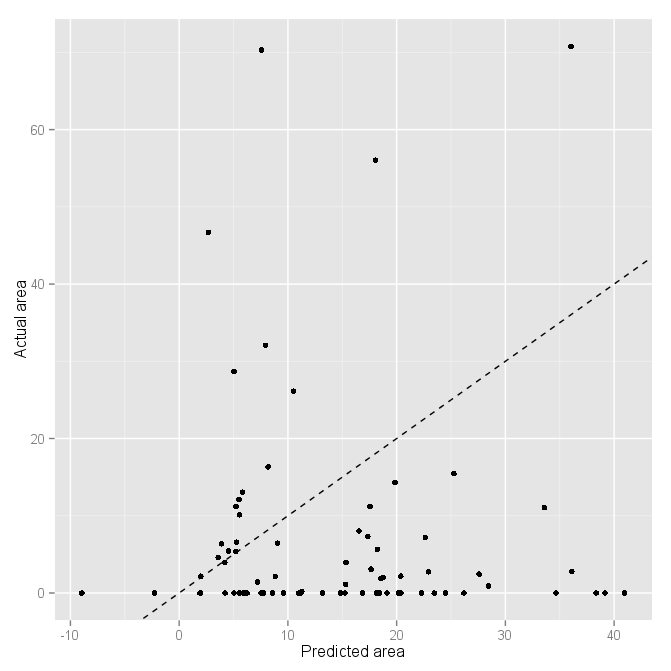
\includegraphics[width=0.4\textwidth]{figures/firenaivepredict.png}
  \caption{Raw data regression---predicted area versus actual area. Dotted line
  is the ideal case of perfect prediction}
\end{figure}

Clearly, our current model is not particularly accurate. In fact, the $R^2$
value for this run evaluates to a mere 0.0001555681. However, it will serve
well as a benchmark for testing the predictive abilities of other models
relative to this one. We now explore some possible transformations and/or
restrictions on the data set in an attempt to improve our predictions.

\subsection{Which data matters?}

We approach the task of narrowing our data range always with our goal in mind:
we are attempting to find the \emph{mean} area given knowledge of a set of
variables. Thus, it would make sense to remove the points which skew the mean
considerably.

The idea we used to break it down involved attempting to find a segment of data
where we have a relatively uniform amount of information for each range of
area. The easiest visual way we could determine this is by trimming down
outliers and showing the distribution of the area until it looks moderately
close to uniform. The difference between the distribution of area in the
original data and our trimmed data is shown in Figures 2 and 3.

\begin{figure}
  \begin{minipage}[b]{0.45\linewidth}
  \centering
  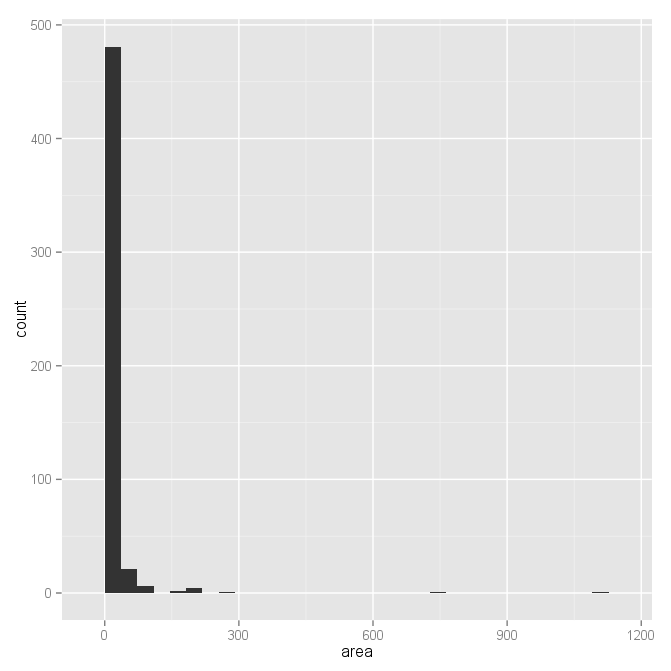
\includegraphics[width=\textwidth]{figures/badhist.png}
  \caption{Distribution of area with raw data}
\end{minipage}
\hspace{0.5cm}
  \begin{minipage}[b]{0.45\linewidth}
  \centering
  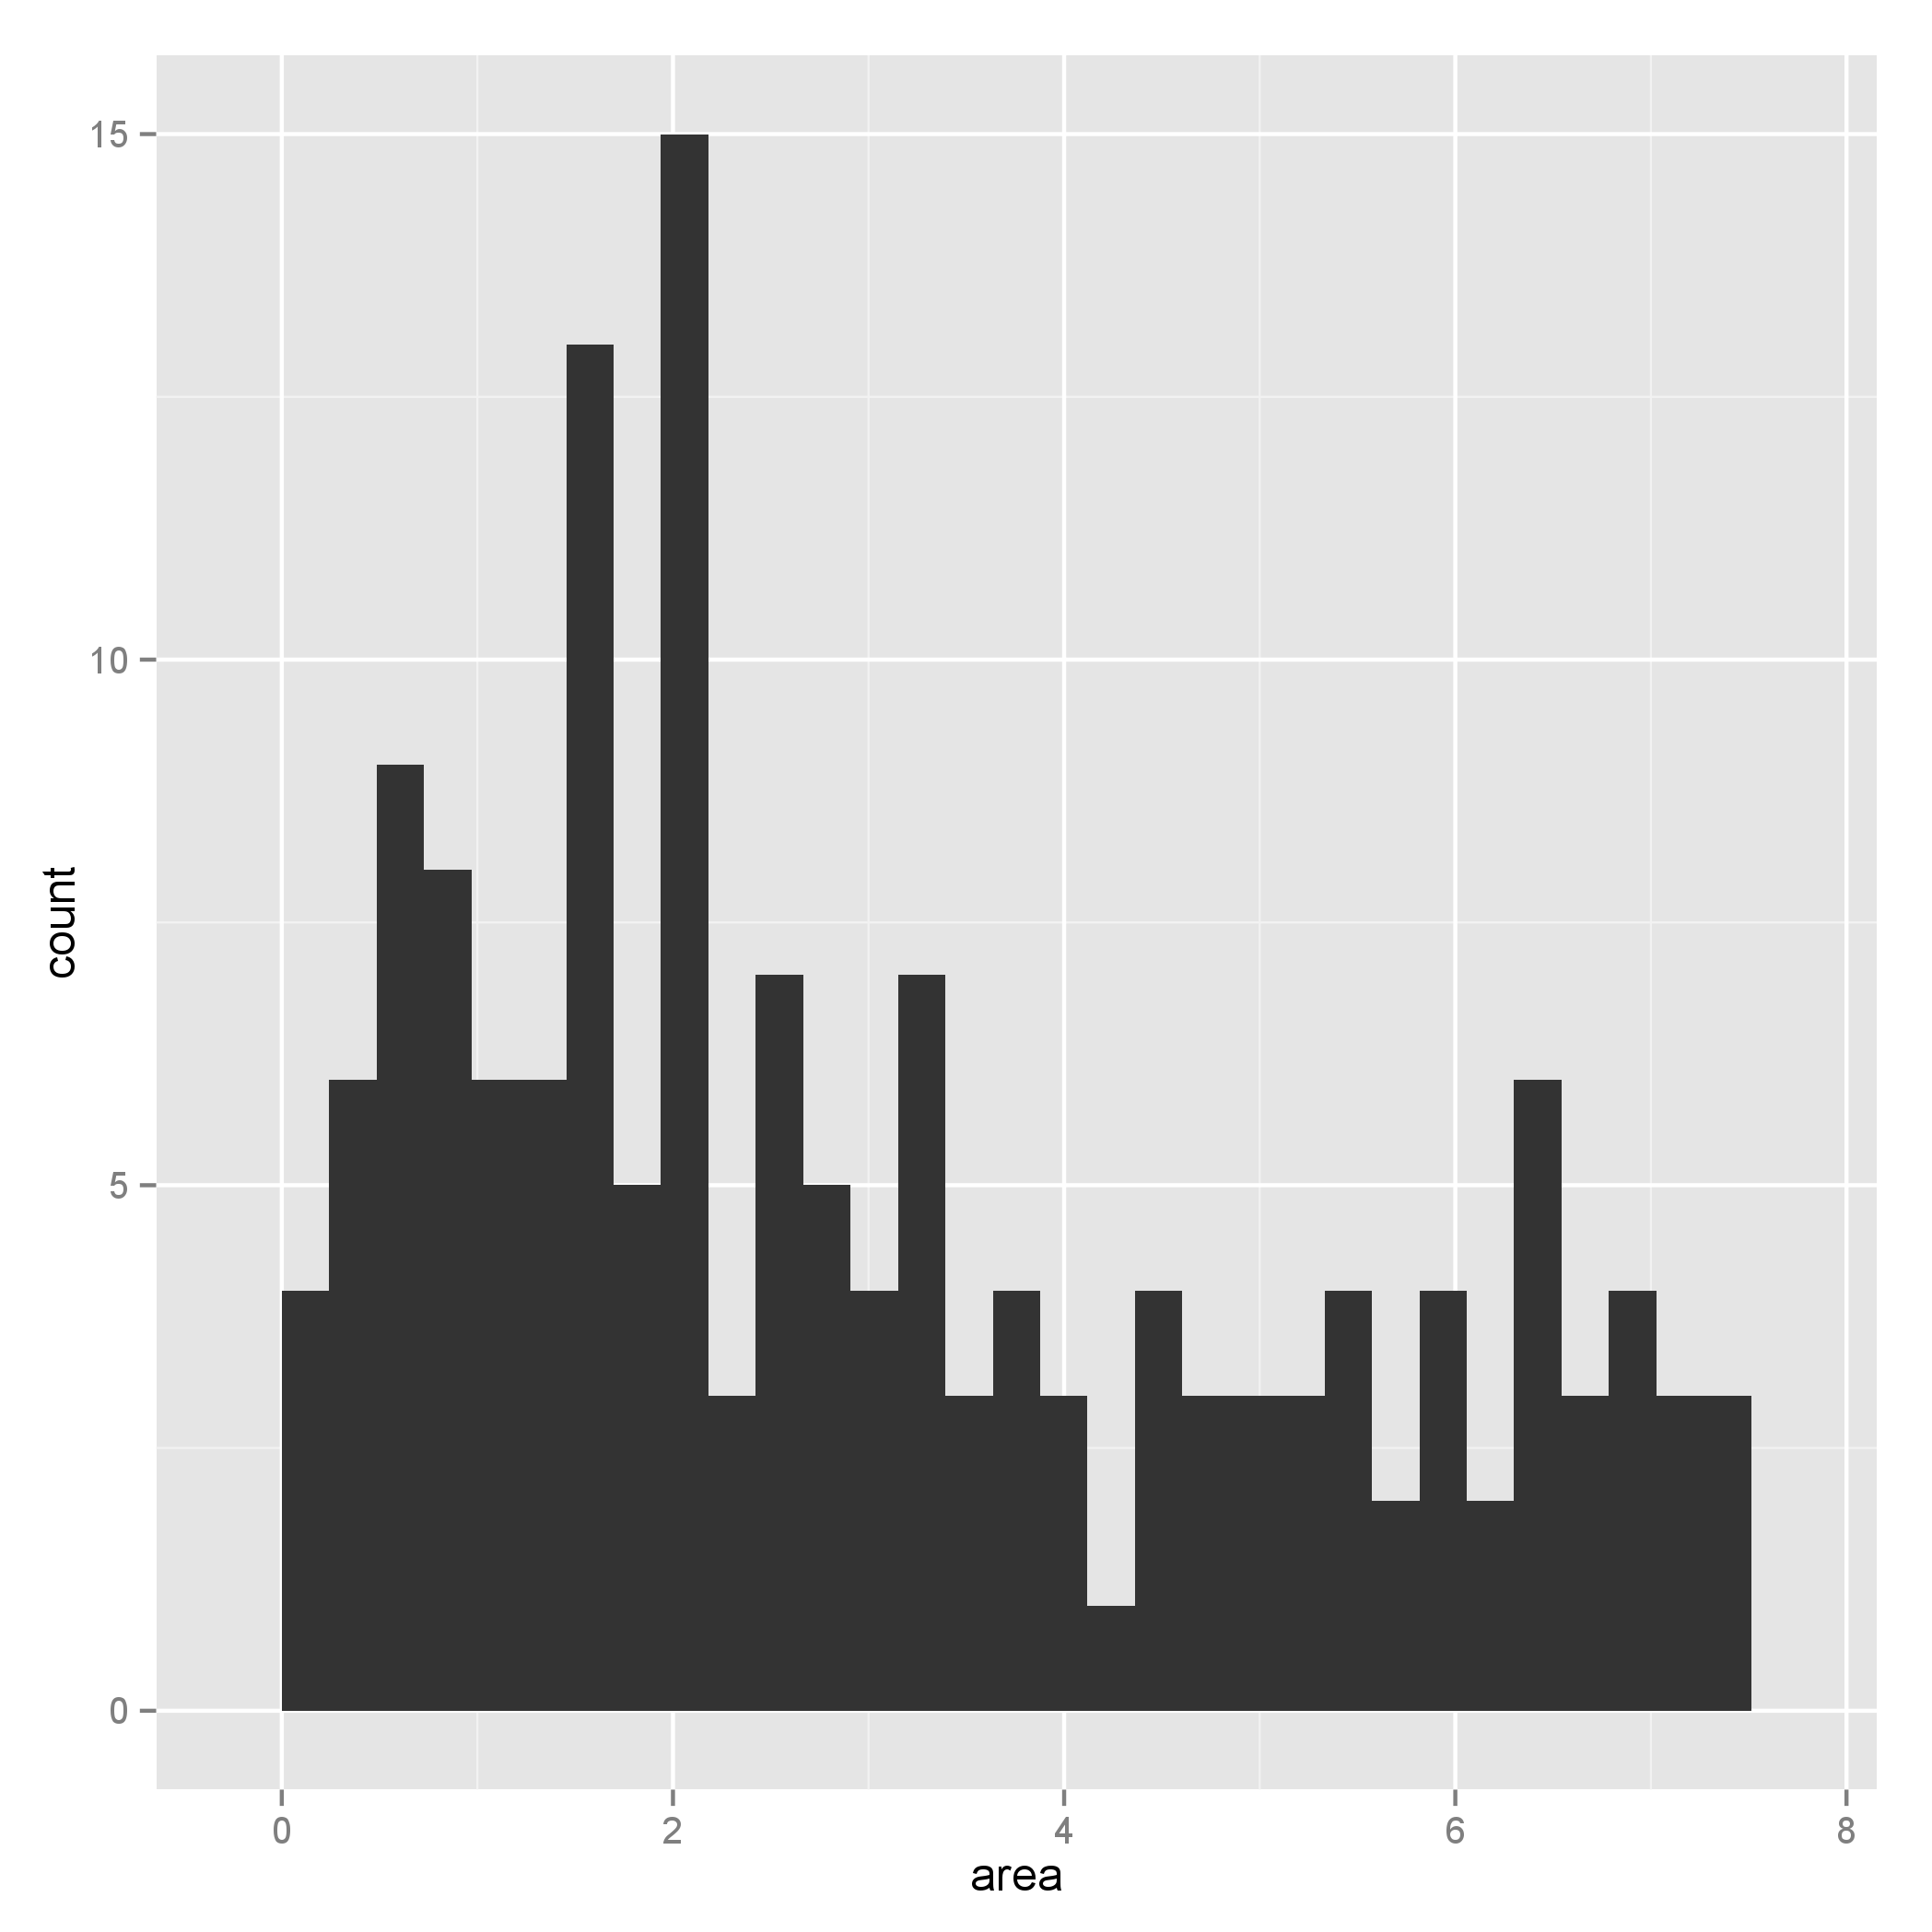
\includegraphics[width=\textwidth]{figures/goodhist.png}
  \caption{Distribution of area with trimmed data}
\end{minipage}
\end{figure}

We continued from this point using two different methods for choosing the
predictors for our smaller data set. The first was to use the forward stepwise
selection process suggested in the project specifications. The second attempt
uses the backward stepwise selection process, which is briefly mentioned in the
textbook. In addition, in the first selection attempt, we transformed the day
and month variables using a sine function with the period equal to the number
of days or months, as suggested by the project writeup. In the second attempt,
these were instead converted to indicator random variables.

\subsection{Predictor Selection 1}

For the second predictor set we decided to use the attributes that are part
of the Fire Weather Index (FWI) such as FFMC, DMC, DC and ISI. 
Before we eliminated part of the data these values did now have a good
$R^{2}$ value compared to the other meteorological data such as temperature,
wind, humidity and rain. However, once we eliminated the data the attributes
that are part of FWI gave us a far better $R^{2}$ value than the other
meteorological variables. Using forward step-wise we started with FWI attributes,
then we tested out different interaction terms between FWI attributes
and found that $DMC \times FMC$  and $DC \times ISI$ greatly increased
the $R^{2}$ of our regression.The only non FWI attribute we decided to
go with was month because we saw a strong correlation between the months
and the area.

\begin{align*}
  \widehat{m}_{area;FFMC,ISI,DC,month,DMC}(t) = &-23.1151201 - 0.2744283 \cdot t_1 + 0.3185786 \cdot t_2 \\
  &+ 0.0122545 \cdot t_3 + 2.5926093 \cdot t_4 \\
  &- 0.2495317 \cdot t_5 - 0.0006686 \cdot t_2 \cdot t_3 + 0.0027410 \cdot t_1 \cdot t_5 	   
\end{align*}
which is obtained from the output of \verb=lm=.

\begin{verbatim}
              		Estimate Std. Error t value Pr(>|t|)    
		(Intercept) 23.1151201  9.0213988   2.562 0.011419 *  
		FFMC        -0.2744283  0.1118159  -2.454 0.015301 *  
		ISI          0.3185786  0.1871206   1.703 0.090799 .  
		DC           0.0122545  0.0035439   3.458 0.000715 ***
		month        2.5926093  0.8779764   2.953 0.003673 ** 
		DMC         -0.2495317  0.1012981  -2.463 0.014935 *  
		ISI:DC      -0.0006686  0.0002937  -2.277 0.024264 *  
		FFMC:DMC     0.0027410  0.0011059   2.479 0.014335 *
\end{verbatim}

With this regression model we got an Adjusted $R^{2}$ value of 0.09632 which
was by far the best value we got at the time. Yet, this is still not a very
good model for predicting the mean area of the fire. So then we decided to try
another method of finding a good predictor set by using the backwards step-wise
approach.

\subsection{Predictor Selection 2}

In our later attempt, we discovered new ways to obtain our set of predictor
variables. First, we settled on a backwards stepwise selection process, where
we begin with all of the first-order predictor variables in our model and
remove, one by one, the variables which show little impact in the regression.
We define ``little impact'' to be a combination of a high p-value and/or a
confidence interval which results in the predictor having close to zero
influence. Second, we replaced the month and day variables with indicators for
each month and day (minus one each in order to avoid linear dependence).  Once
the set is trimmed to a reasonable level, interaction terms are added and
Adjusted $R^2$ value is monitored. If an interaction term increases Adjusted
$R^2$, we keep it, otherwise it is thrown out. 

Naturally, the danger in this stage is in adding too many terms. According to
the text, a good rule of thumb is that the number of predictors be less than
the square root of the number of data points. In our limited data set, we have
a total of 153 points to work with, meaning that there should be twelve or
fewer predictors. We strayed on the conservative side, and left out some
predictors which only brought a modest increase in Adjusted $R^2$. This left us
with the final set, as seen in the output of \verb=lm=:

\begin{verbatim}
Coefficients:
             Estimate Std. Error t value Pr(>|t|)    
(Intercept)  4.880875   0.660986   7.384 1.16e-11 ***
X           -0.149919   0.069056  -2.171 0.031584 *  
DC           0.004469   0.001830   2.442 0.015821 *  
June        -2.632148   1.043833  -2.522 0.012778 *  
July        -9.321820   2.764645  -3.372 0.000961 ***
August      -3.541709   1.104434  -3.207 0.001656 ** 
September   -3.756403   1.250390  -3.004 0.003145 ** 
ISI         -0.079231   0.047007  -1.686 0.094070 .  
DC:July      0.009353   0.004713   1.984 0.049124 *  
ISI:July     0.345872   0.181849   1.902 0.059186 .  
\end{verbatim}

This can be further solidified in mathematical form:
\begin{align*}
  \widehat{m}_{A;V}(t) = &4.880875 - 0.149919 \cdot t_1 + 0.004469 \cdot t_2 \\
                         &- 0.079231 \cdot t_3 - 2.632148 \cdot t_4 \\
                         &- 9.321820 \cdot t_5 - 3.541709\cdot t_6 \\
                         &- 3.756403\cdot t_7 + 0.009353\cdot t_2 t_5 
                         + 0.345872\cdot t_3 t_5
\end{align*}
where $A$ is the area, $V$ is the vector (X, DC, ISI, June, July, August, 
September) and $t$ is the vector of inputs corresponding to each position in 
the $V$ vector.

Using this set, the Adjusted $R^2$ is reduced to 0.1456---a huge improvement
over the previously used predictors.

%\subsection{Final predictor set}
%
%After testing various predictor selection methods, we came up with the following predictor set:
%\begin{itemize}
%	\item FFMC
%	\item ISI
%	\item DMC
%	\item Month
%	\item DC
%	\item DC:ISI
%	\item DMC:FFMC
%\end{itemize}

\subsection{Cross validation}

While the Adjusted $R^2$ value from \verb=lm= is a useful indication of the fit
of a model to the data it was built from, what we are really looking for is the
power of the model to predict future outcomes. This prediction capability can
be verified using cross validation. For this, we created a function named
\verb=cvlm=, which randomly splits an input data frame into training and
testing sets of a specified size, runs \verb=lm= on the training set, predicts
the outcome of the testing set, and combines those outcomes with the real data
in a matrix. We can then use this matrix for plotting and also for computing
$R^2$. We chose to run \verb=cvlm= with 110 points for the training set and the
remaining 43 for the testing set. The results of this run can be seen in
Figure~\ref{fig:linreggood1}. The mean $R^2$ value over two thousand runs of
\verb=cvlm= turned out to be 0.1194353.

To further test the robustness of our model, we also created a second cross
validation function---\verb=cvlmmore=---to test our model built on the
restricted data set against the raw data. Each time we tested our model against
150 points from the raw data collection. One run of this function can be seen
in Figure~\ref{fig:linreggood2}. Not surprisingly, the mean $R^2$ value over
two thousand runs of \verb=cvlmmore= is significantly lower, at 0.005969264.

\begin{figure}
  \begin{minipage}[b]{0.45\linewidth}
  \centering
  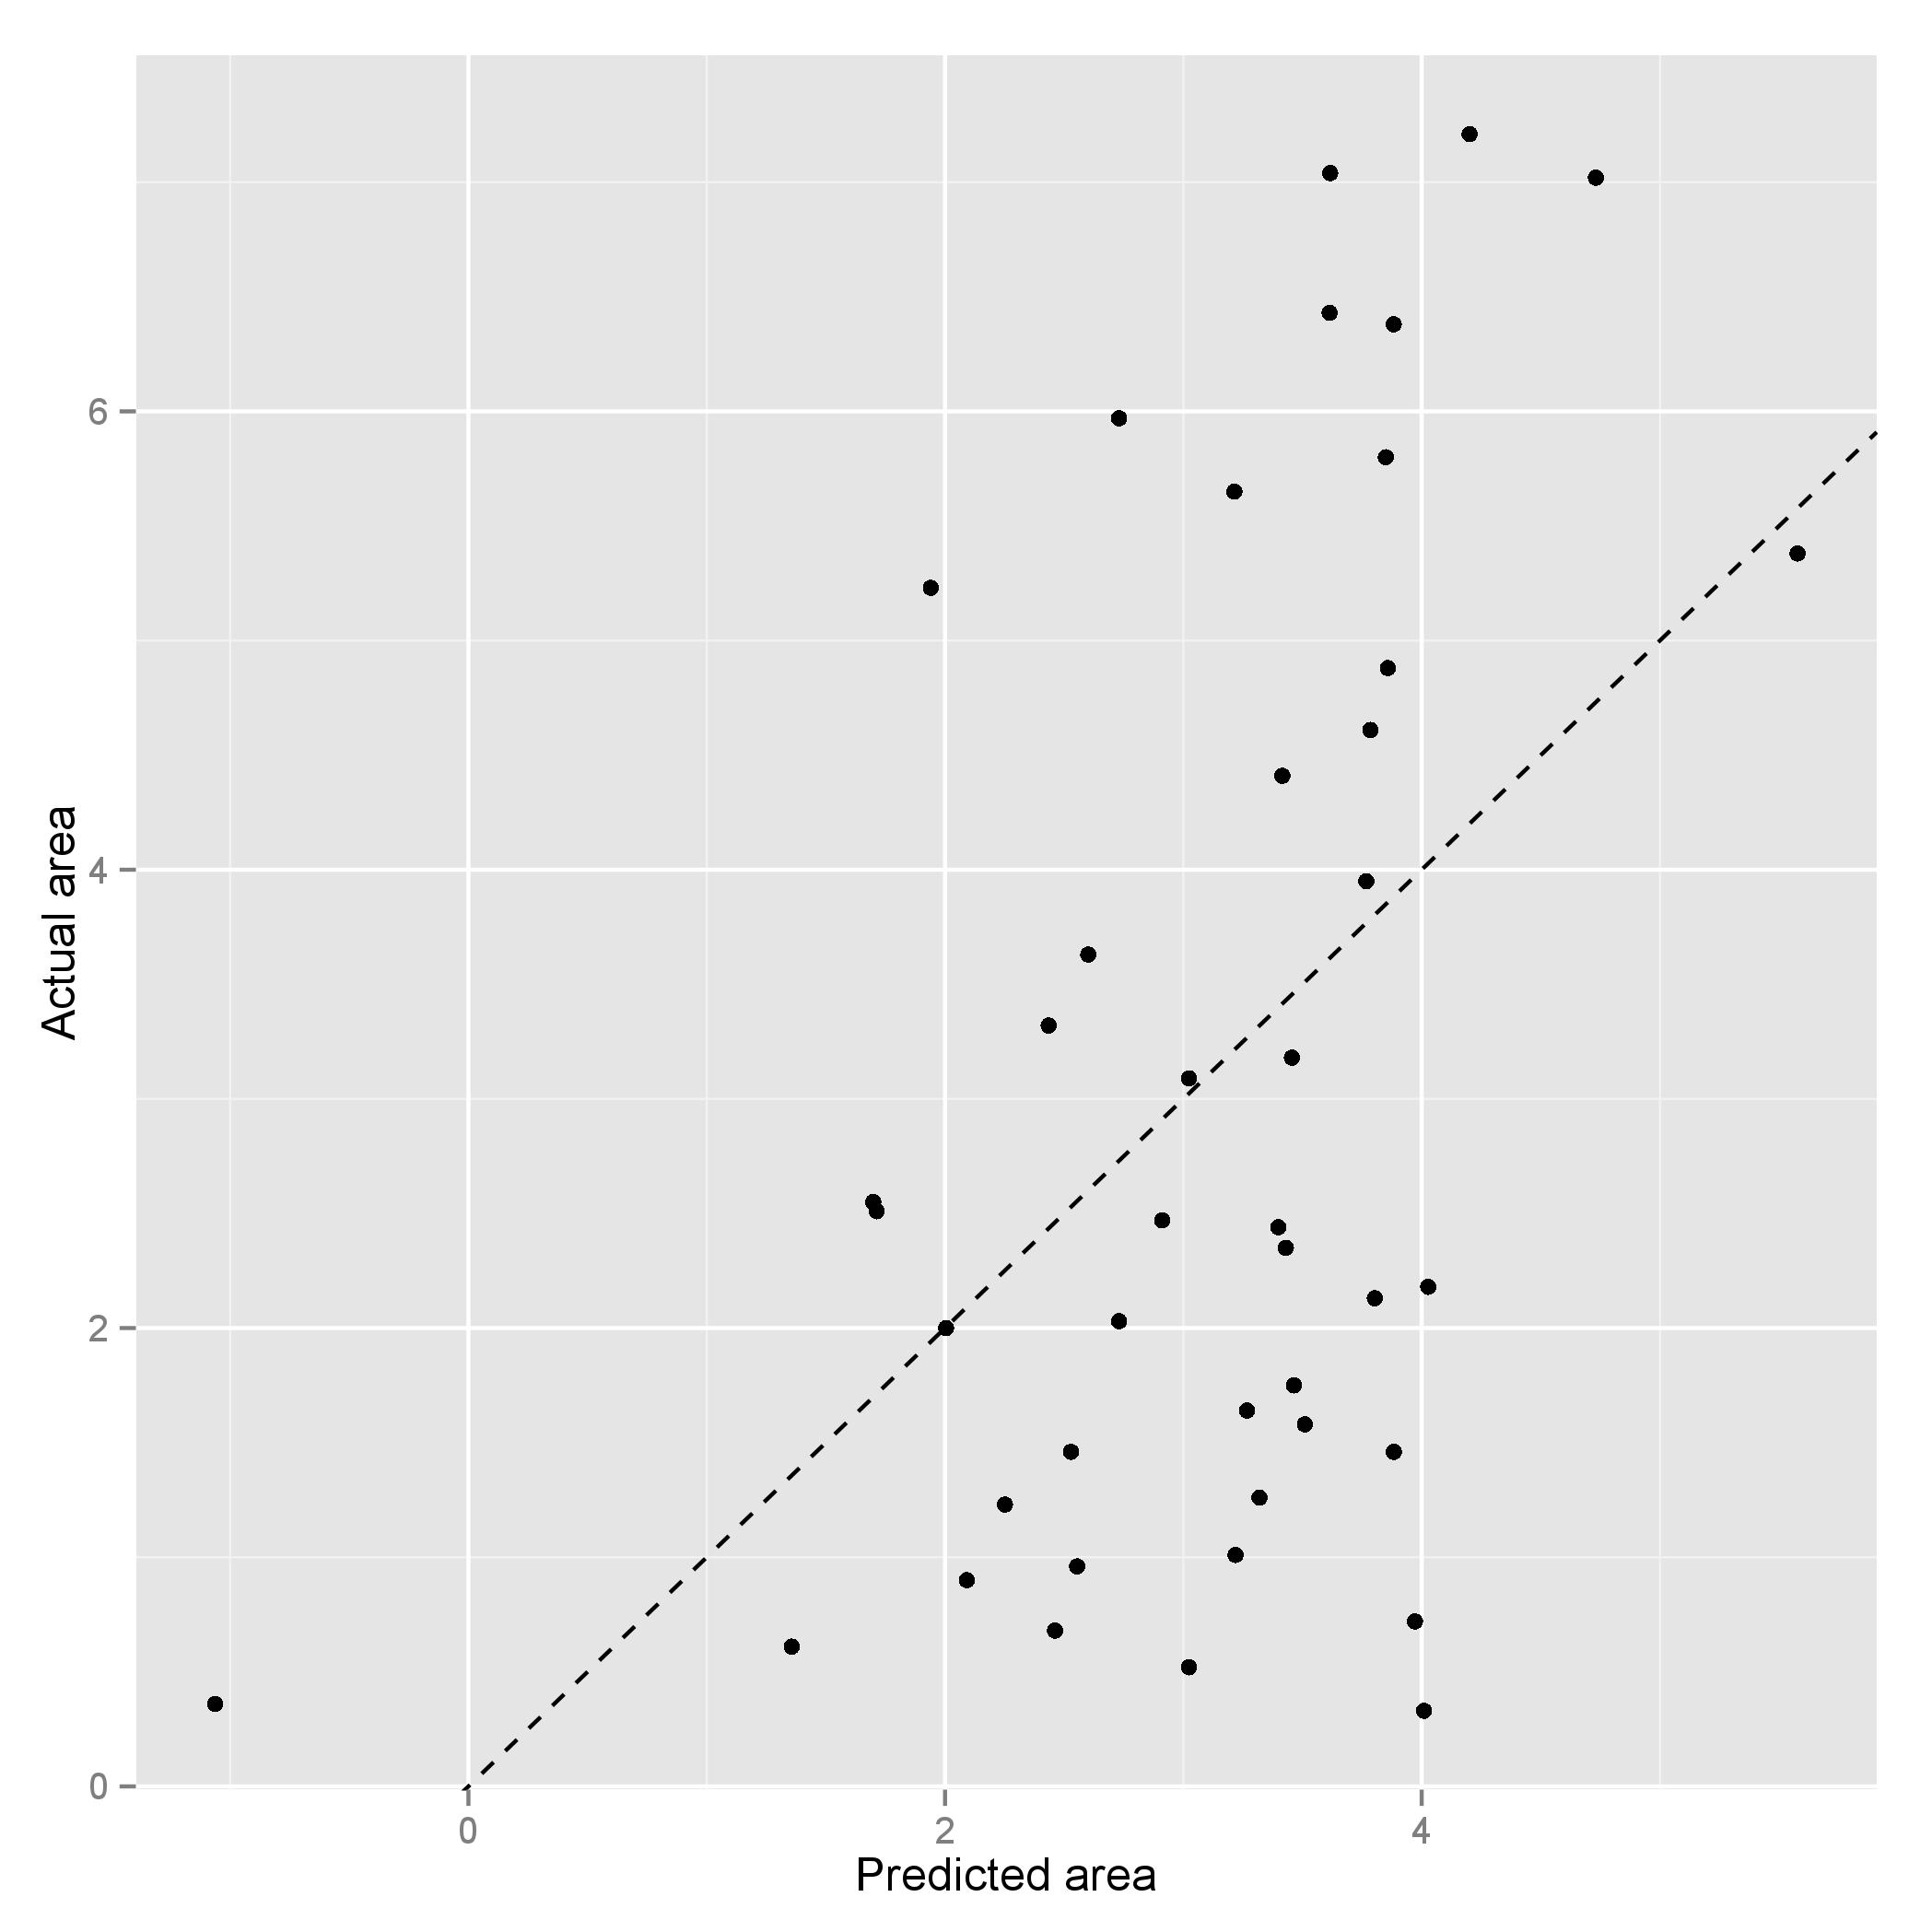
\includegraphics[width=\textwidth]{figures/goodfiresowndat.png}
  \caption{Actual area vs.\ predicted area with best regression model on
  trimmed data set}
  \label{fig:linreggood1}
\end{minipage}
\hspace{0.5cm}
  \begin{minipage}[b]{0.45\linewidth}
  \centering
  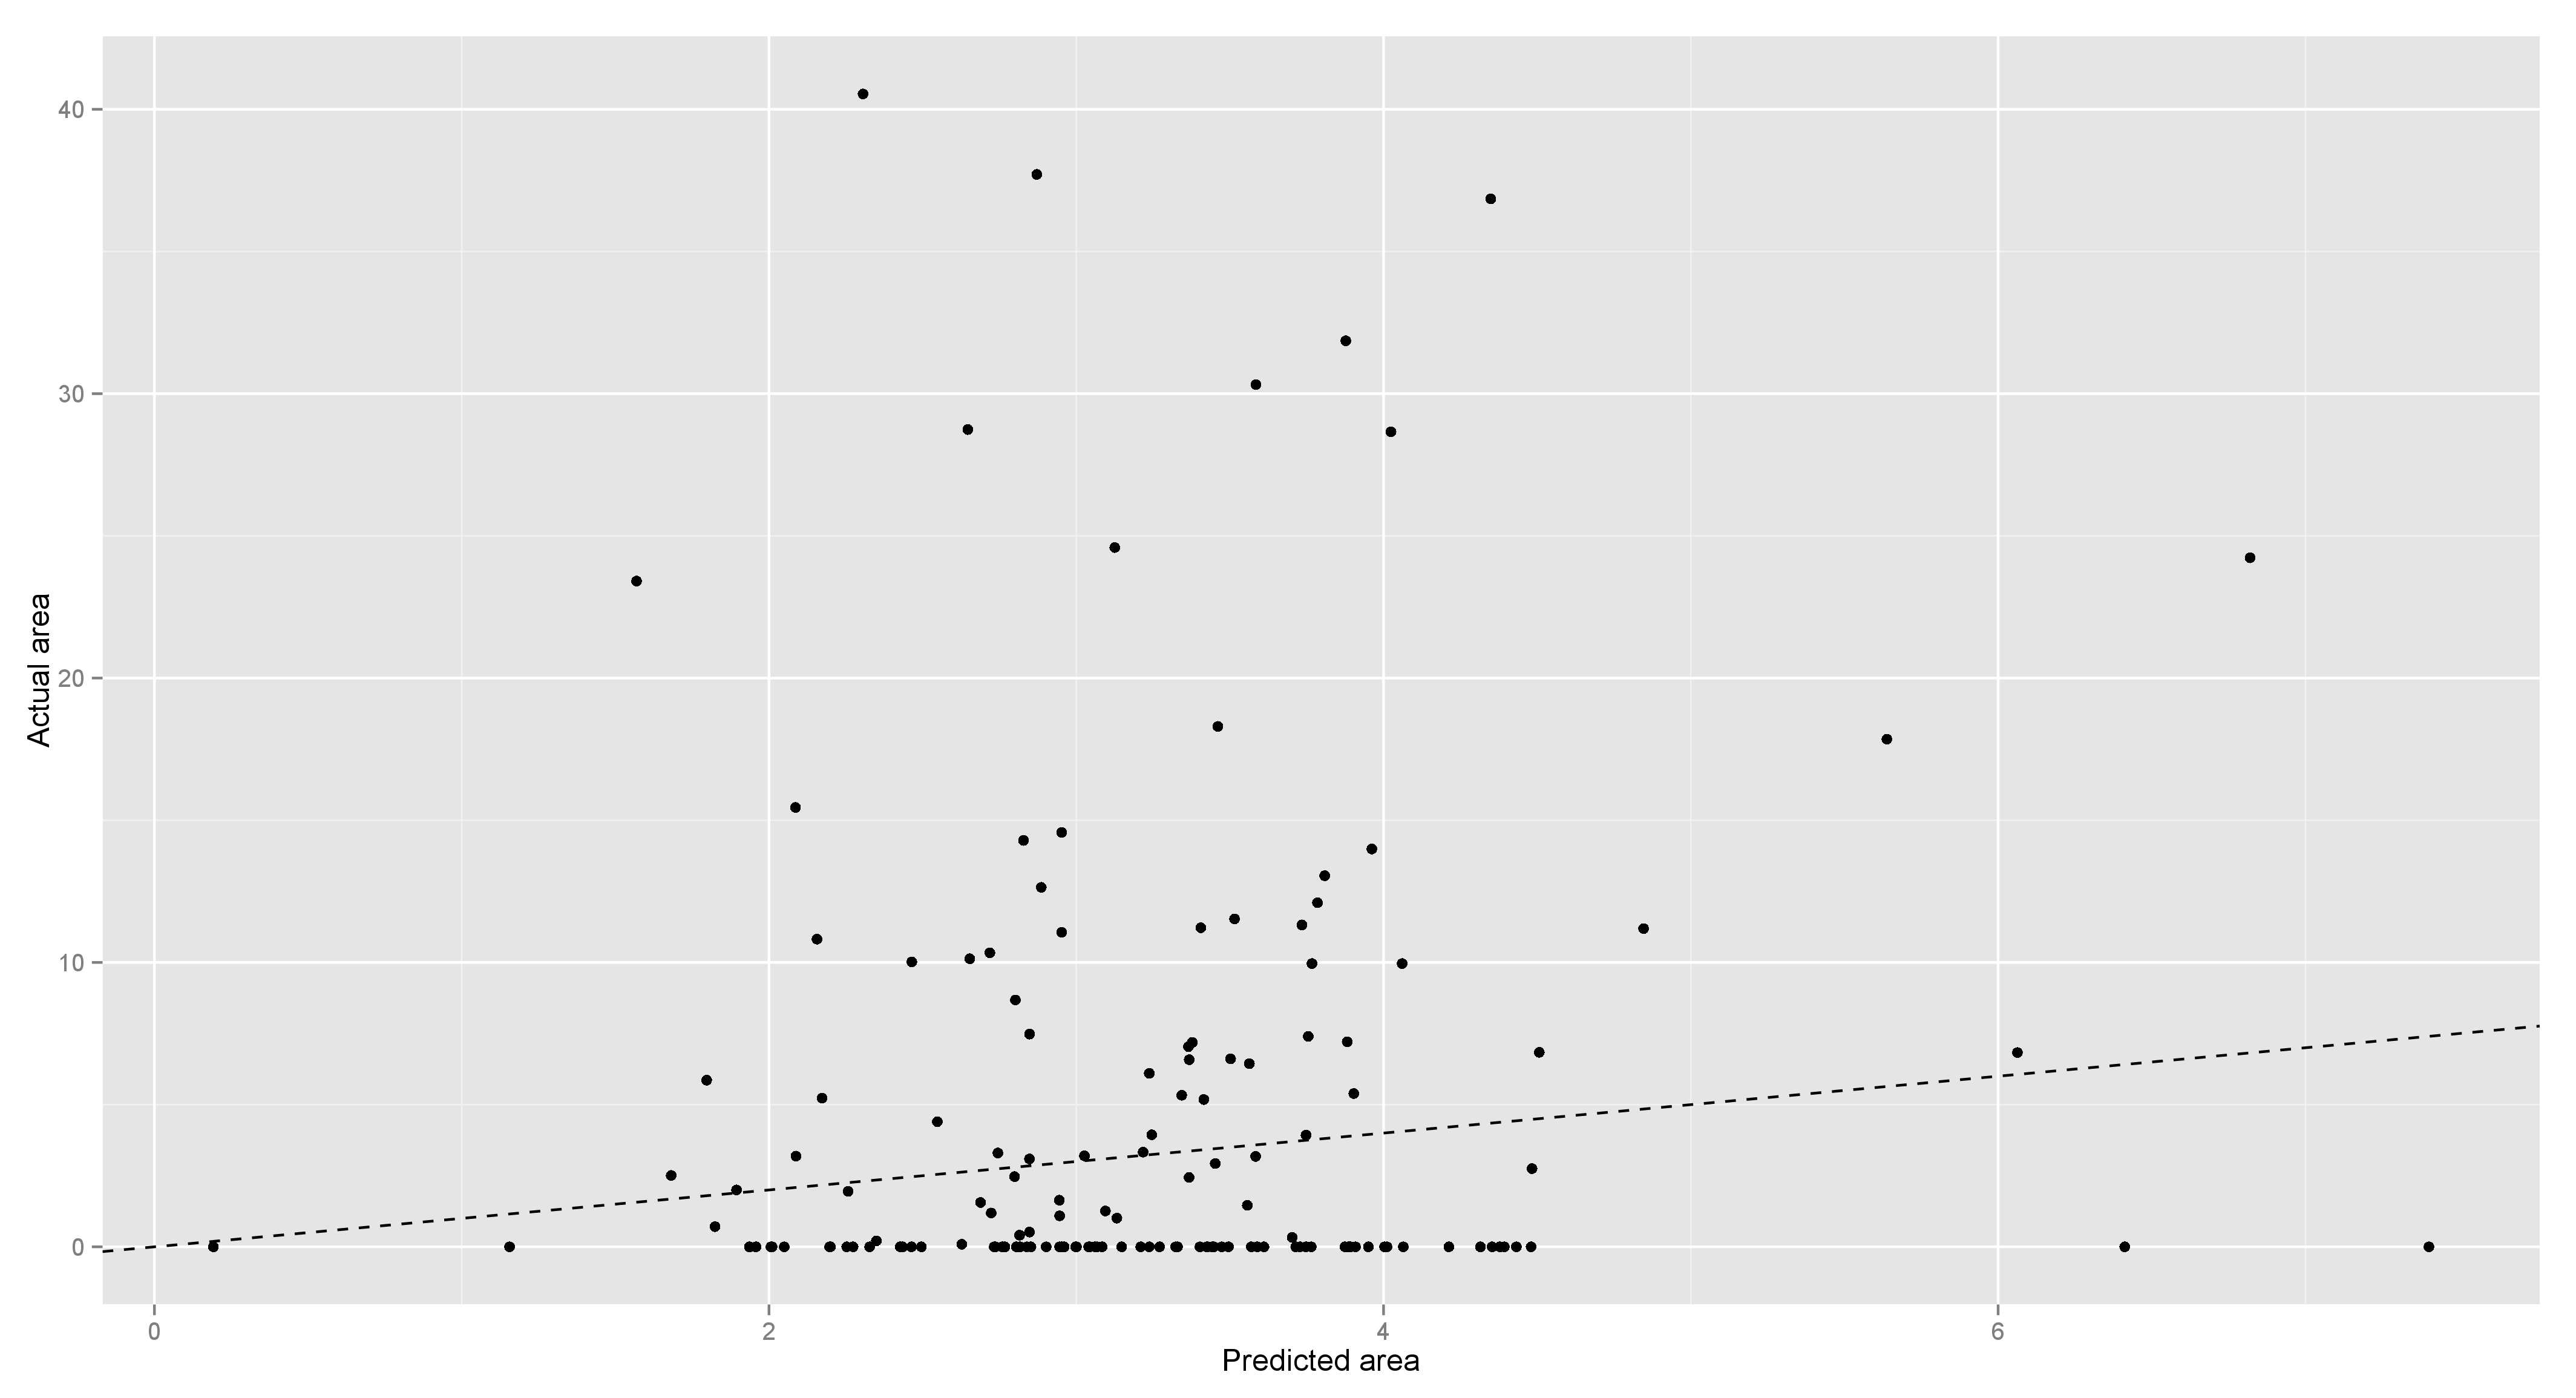
\includegraphics[width=\textwidth]{figures/goodfiresalldat.png}
  \caption{Actual area vs.\ predicted area with best regression model on raw
  data set}
  \label{fig:linreggood2}
\end{minipage}
\end{figure}

%--------------------

\subsection{Multicollinearity}

In a situation with many predictor variables, as we have, we have the risk of
multicollinearity. Detecting and dealing with multicollinearity can help
improve the accuracy of the model and the selection of predictor variables. One
common method of detecting multicollinearity is through a condition number---a
concept alluded to in section 14.17.4 in the book. Through a quick Internet
search, we found that the condition number is formally defined as
\begin{equation*}
    \kappa = \sqrt{ \frac{ \lambda_{\text{max}}}{\lambda_{\text{min}}}}
\end{equation*}
where $\lambda_{\text{max}}$ is the largest eigenvalue of the correlation
matrix of the predictors and $\lambda_{\text{min}}$ is the smallest. A rough
rule of thumb, according to the textbook, is that $\kappa$ should be less than
15 if there are no major multicollinearity problems.

Conveniently, R has a built-in function to compute this value for us---the
\verb=kappa= function. Using R's \verb=cor= function, we created the
correlation matrix from our predictor vectors, and input the result into
\verb=kappa=. The number returned was 107.1714. Looking over the correlation
matrix ourselves, we saw a relatively high correlation between some variables,
for example, September and DC. Removing these variables would be a problem for
us, since we already determined that these were the variables critical to a
reasonable $R^2$. However, the side effect of multicollinearity, as described
in the textbook, is large standard errors. Looking back at the output from
\verb=lm=, we see that the standard errors are not drastic. We can conclude
from this that we should not worry about the multicollinearity in our model.


\subsection{Nonparametric methods}

For our nonparametric analysis, we used the provided k-nearest neighbor
function. We return to our original, completely intact data, to attempt
regression with the nonparametric technique, using the same predictors we
discovered initially. To aid in our inquiry, we created two functions:
\verb=cvknn= and \verb=cvknnmore=. The former performs cross validation by
training on some portion of the input data and validating on the rest. The
latter takes two data sets as input: one for training and one for validating.
They both generate output in a form useful for both plotting and finding $R^2$.

Applying \verb=cvknn= to our whole data set with our original predictors
produced an almost sinusoidal $R^2$ for increasing $k$. This can be seen in
Figure~\ref{fig:r2knn}. The shape of the plot seems unusual, however, it
makes sense given some thought. Because the data is nearly random, picking a
small number of nearest neighbors could still be off by a substantial margin.
On the other hand, averaging too many neighboring values will force the mean to
a certain value for any input. This creates a sweet spot for $k$, which can be
seen in the peak in the graph.

Next, we ran \verb=knn= with the best predictors from the smaller data set. In
the first trial, we ran our cross validation between subsets of the smaller
data set using \verb=cvknn=. We sampled the mean $R^2$ values for $k=1,5,10,15$
with 110 samples in the training set and the rest in the validation set over
2000 iterations. $R^2$ did not appear to change substantially as $k$ increased,
changing from 0.01875791 at $k=1$ to 0.02237041 at $k=15$.
Figure~\ref{fig:r2knn} shows the change in $R^2$ as $k$ increases.

Out of curiosity, we also ran the cross validation with the smaller data as the
training set and the whole data as the validation set. This employed the use of
\verb=cvknnmore=. What is odd about this case is that it predicts areas for
low $k$ better than the model using the whole data for training. Considering
the majority of data has a relatively low area value and the training set also
consists of observations with a small area, this \emph{could} be explained by
the lack of outliers in this model.

\begin{figure}
  \centering
  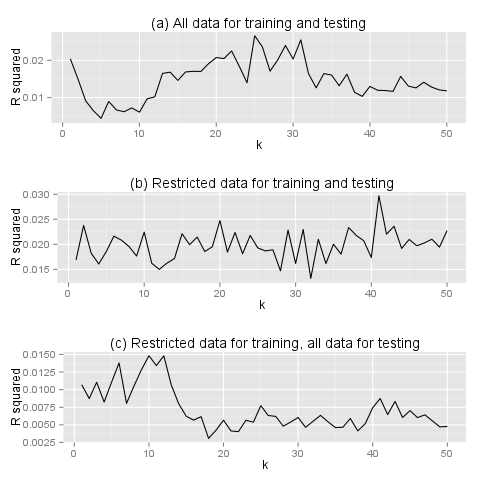
\includegraphics[width=0.4\textwidth]{figures/r2knn.png}
  \caption{$R^2$ plotted against $k$ for three sets of k-nearest neighbor
  regressions}
  \label{fig:r2knn}
\end{figure}

\subsection{Further possibilities}

Initially, doing variations and correlations between predictor variables and the response
variable resulted in abnormally low values. This led us to consider what the forest looked like.
We did this by creating a \verb+frequencyGrid+ and \verb+areaGrid+ that corresponds to each
of X,Y coordinates that exist. The data is as shown below:

\begin{figure}
  \begin{minipage}[b]{0.475\linewidth}
  \centering
  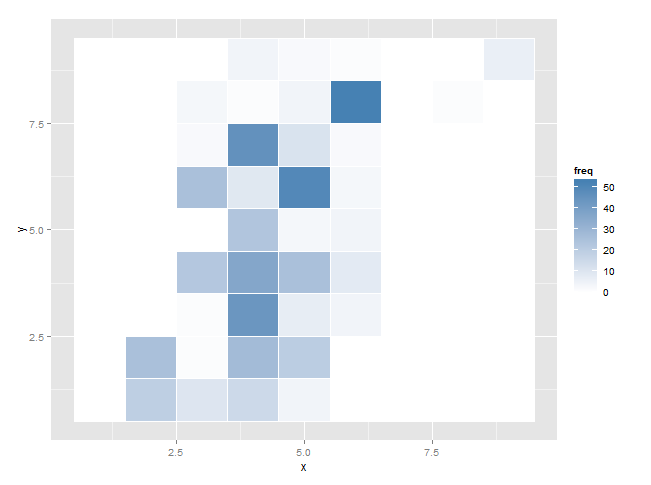
\includegraphics[width=\textwidth]{figures/freq.png}
  \caption{Frequency grid of forest data}
\end{minipage}
\hspace{0.5cm}
  \begin{minipage}[b]{0.475\linewidth}
  \centering
  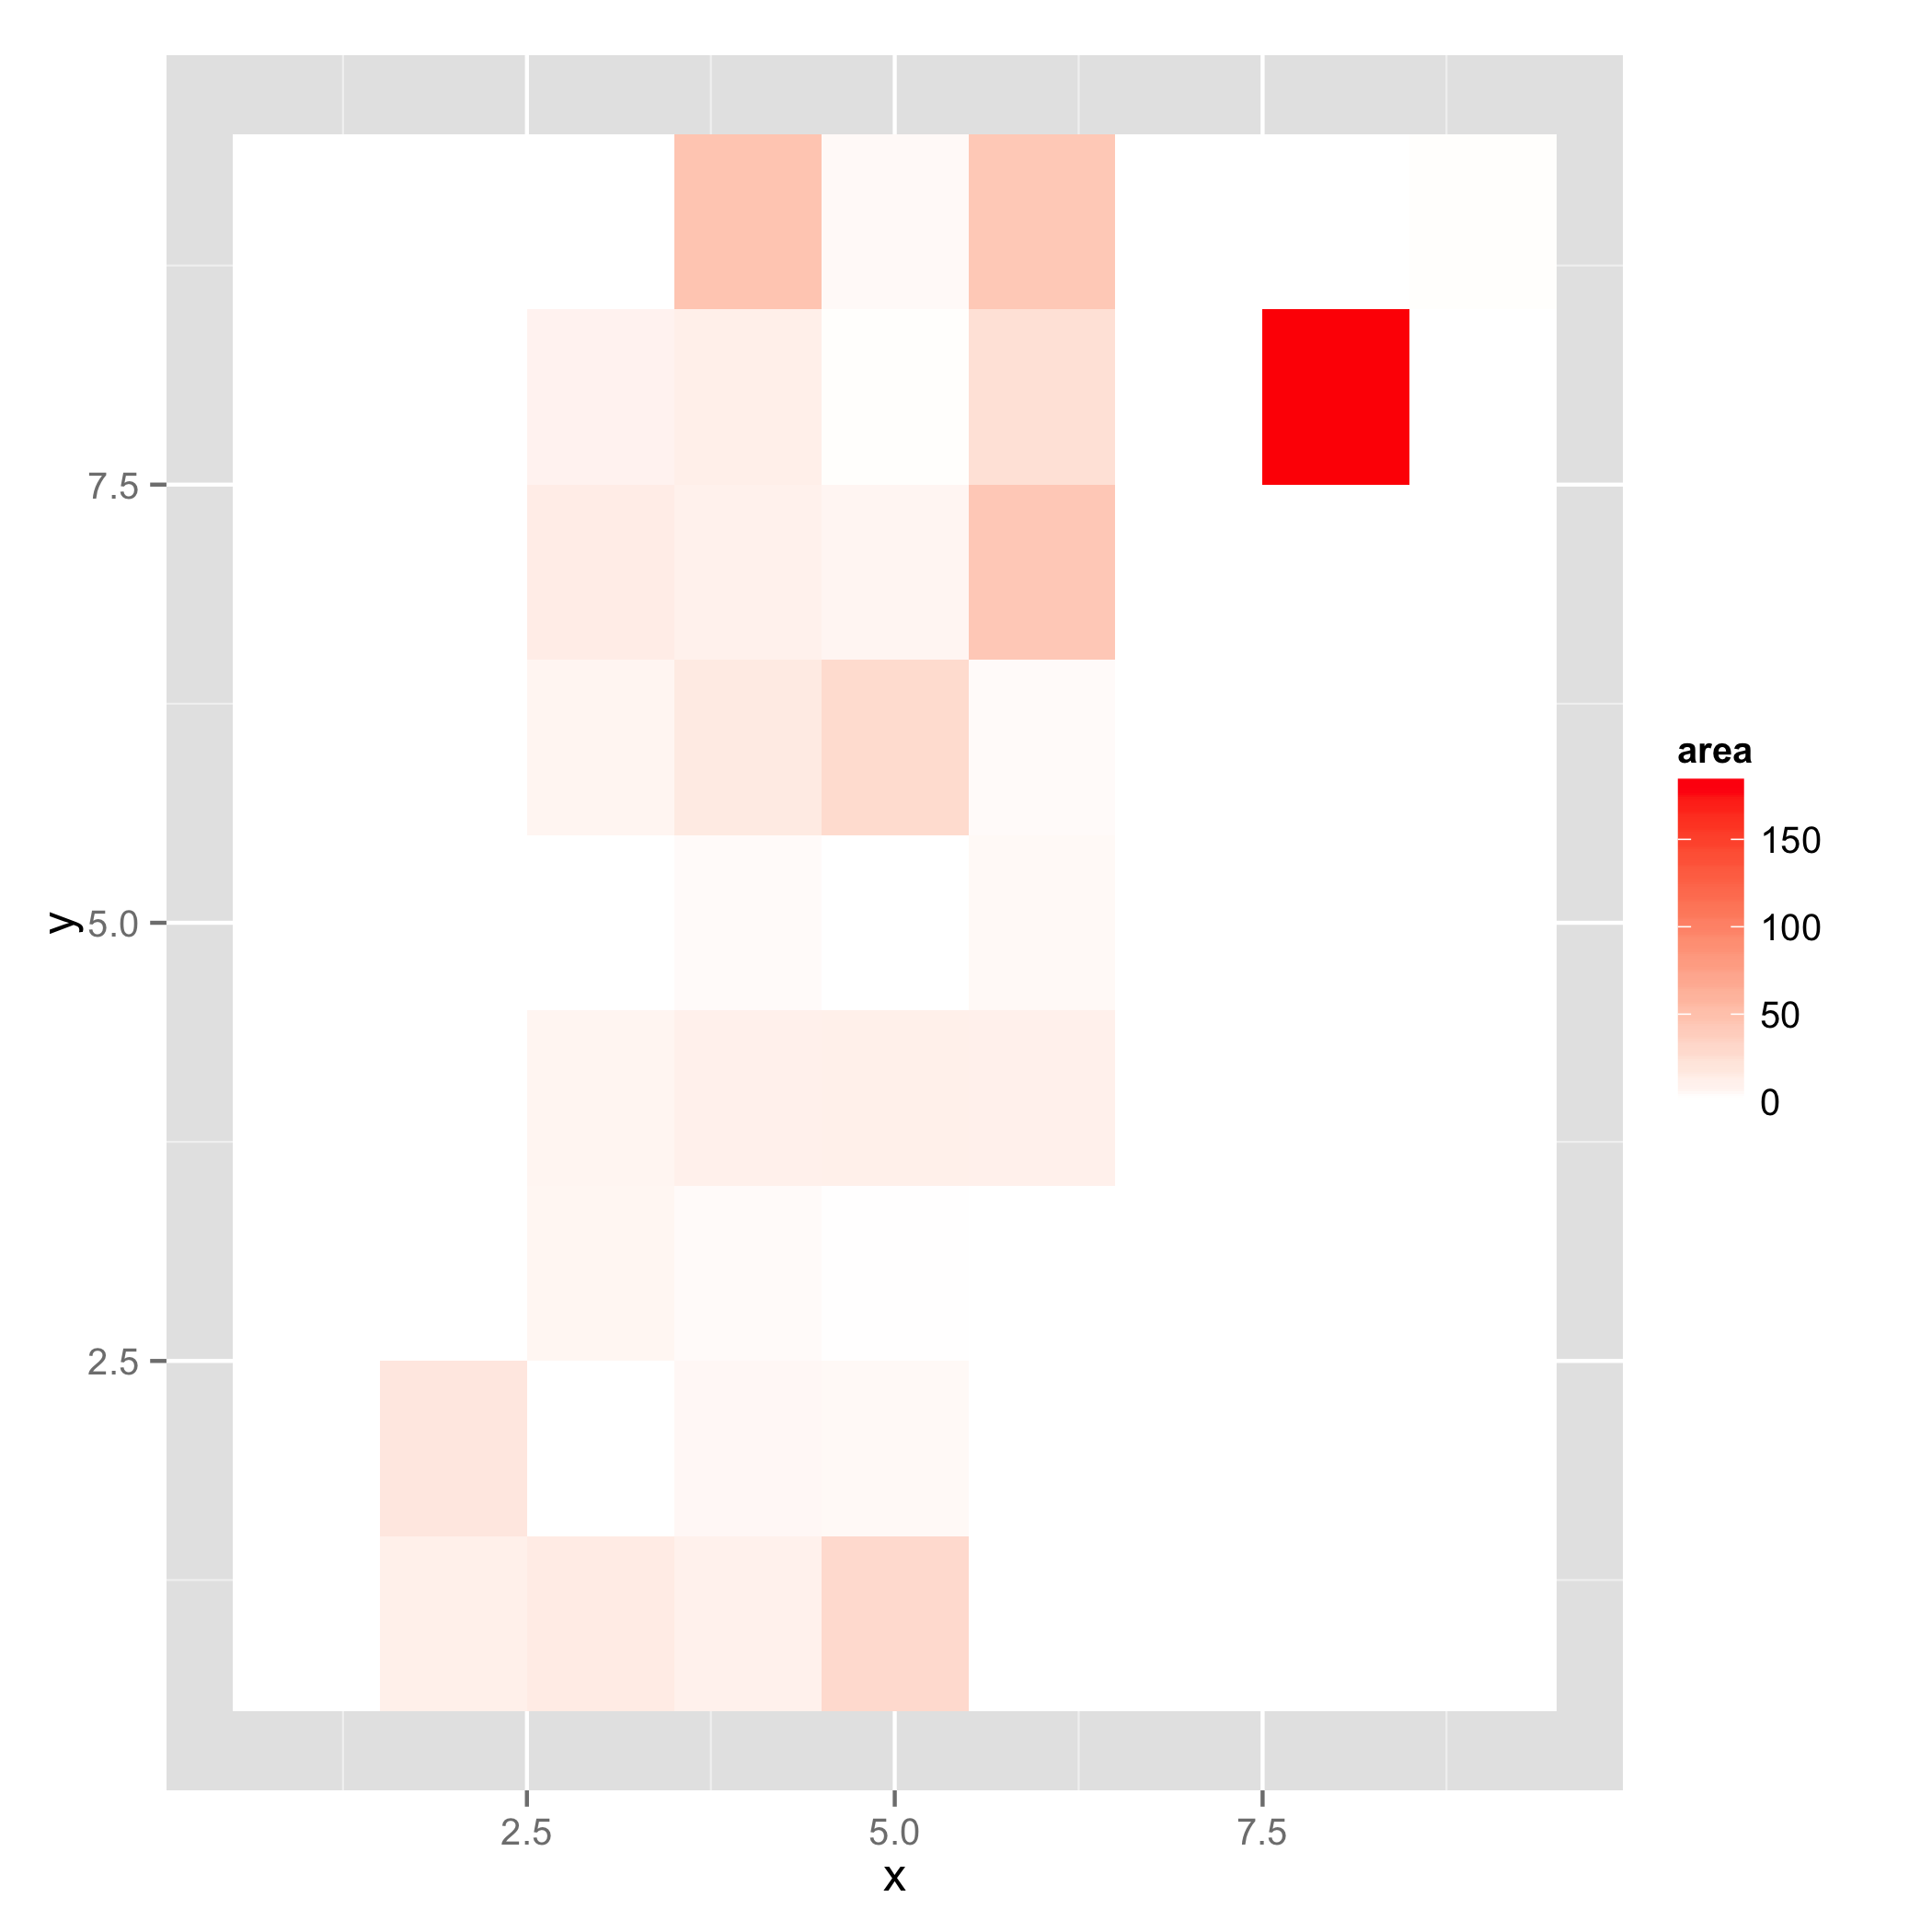
\includegraphics[width=\textwidth]{figures/area.png}
  \caption{Area grid of forest data}
\end{minipage}
\end{figure}

\verb+frequencyGrid+ (Figure 6) and \verb+areaGrid+ (Figure 7) reveal several
trends about the forest:

\begin{enumerate}
	\item $\approx 44\%$ of the forest locations never had a fire
	\item Locations with many fires usually have small mean areas
	\item Locations with few fires usually have large mean areas
\end{enumerate}

These trends suggested that certain parts of the data set were
irrelevant to our prediction of fire area. In order to more accurately
predict fire size in places that actually had fires, data that corresponds
to X,Y coordinates with a mean area of NaN or frequency of 0 can be ignored.
However, this task is beyond the scope of this project.

\section{Parkinson's disease}

The dataset was created by Max Little of the University of Oxford, in
collaboration with the National Centre for Voice and Speech, Denver, Colorado,
who recorded the speech signals. The main aim of the data is to discriminate healthy
people from those with PD, according to "status" column which is set to 0 for
healthy and 1 for PD. Our goal with this data is to try to monitor patients with
Parkinson's disease remotely, by simply analyzing their voices on the phone.

\subsection{Possible Predictors}
The first variable we looked at to see if it could be a good predictor variable was
MDVP.Fo.Hz. We ran the following code to get a generalized linear model:

\begin{verbatim}
glm(formula = parkinson$status ~ parkinson$MDVP.Fo.Hz., family = binomial)
\end{verbatim}

From this we got the following output:

\begin{verbatim}
                       Estimate Std. Error z value Pr(>|z|)    
(Intercept)            4.706084   0.775185   6.071 1.27e-09 ***
parkinson$MDVP.Fo.Hz. -0.022051   0.004446  -4.960 7.05e-07 ***
\end{verbatim}

We then found the mean value of MDVP.Fo.Hz when the status was zero and got a mean of
181.9378 then we found the mean value if the status was one which was 145.1808. After
we got these values we used the logistic equation and plugged the intercept value, the
$\hat{\beta}$ and first the mean of MDVP.Fo.Hz when the status is zero to get a value of
0.6668947 which is not a good value for status of zero since we need it to be $\leq$ 0.5.
We did the same thing but now using the mean of MDVP.Fo.Hz with status one and got
a value of 0.8182747 which is higher than 0.5 but since the value that we got for
status zero was bad we decided not to use this as one of our predictor variable.

We repeated these steps for the other variables and came up with the following data:

\begin{table}[h]
  \centering
\begin{tabular}{|l|c|c|c|c|c|c|}
\hline
name & intercept & $\hat{\beta}$ & mean0 & mean1 & logit0 & logit1 \\
\hline
MDVP.Fhi.Hz. & 1.871388 & -0.003694 & 223.6368 & 188.4415 & 0.6668947 & 0.8182747 \\
\hline
MDVP.Flo.Hz. & 3.476248 & -0.019075 & 145.2073 & 106.8936 & 0.6696094 & 0.8080288 \\
\hline
MDVP.Jitter.Abs. & -1.0556 & 66665.3255 & 2.3375e-05 & 5.068027e-05 & 0.6230941 & 0.9107654 \\
\hline
spread1 & 15.8608 & 2.3966 & -6.759264 & -5.33342 & 0.416196 & 0.9560066 \\
\hline
spread2 & -2.4283 & 17.5354 & 0.160292 & 0.2481327 & 0.5944722 & 0.9996633 \\
\hline
PPE & -4.2214 & 32.2906 & 0.1230171 & 0.2338282 & 0.438044 & 0.9654122 \\
\hline
NHR & 0.4717 & 39.8604 & 0.01148271 & 0.02921095 & 0.7169546 & 0.8369981 \\
\hline
MDVP.Shimmer.dB & -1.497 & 12.353 & 0.1629583 & 0.3212041 & 0.6262175 & 0.9220717 \\
\hline
HNR & 7.0326 & -0.2576 & 24.67875 & 20.97405 & 0.662701 & 0.8361264 \\
\hline
RPDE & -2.4316 & 7.4058 & 0.4425519 & 0.5168159 & 0.699696 & 0.8015222 \\
\hline
DFA & -6.151 & 10.233 & 0.6957156 & 0.7254079 & 0.7247721 & 0.7811019 \\
\hline
\end{tabular}
\end{table}

Looking through these values we can see that spread 1 and PPE are the only
ones that satisfy the condition in which we want logit of status zero to
be $\leq$ 0.5 and logit of status 1 to be $<$ 0.5. This helped us start to
figure out the predictor set by first including PPE and spread 1.

\subsection{Predictor Selection 1}

After choosing PPE and spread 1 as our predictor variables, we went ahead and
ran cross-validation to figure out if the predictor set of both of them
together is any good. Using our cross-validation function \verb+cvglmprop+
that is included in p2.R which returns the proportion of cases that were
predicted correctly, and found that we correctly predicted a patient's
status 85.12577\% of the time.

We then tried each predictor variable by themselves and ran cross-validation
on that model. First, using PPE we got that 85.46082\% we are predicting
correctly. This is better than using both predictor variables together as
we did in the previous cross-validation. Then, we ran cross-validation on
the model with just spread 1 as the predictor variable and we got that 85.4732\%
we are predicting correctly. After looking at this we decided that using
spread 1 or PPE separately was better than using them together and settled
that spread 1 was the predictor variable we are going to use for our model.
However, before we continued we wanted to see if using spread 1 and PPE together
with a mix of interaction variables could improve our model.

\subsection{Predictor Selection 2}

We first tried to add the interaction term $PPE \times spread 1$ to our model
and ran it through the cross-validation and got 84.97113\% the model predicted
correctly which is worse than we had before. Then, we thought adding $spread1^{2}$
as the interaction term might lead to better results but again we did not see
improvement with 85.11031\% predicted correctly. We then went ahead and
tried $PPE^{2}$ as an interaction term and the model predicted 85.02371\% correctly.

\subsection{Final predictor set}

After testing various predictor selection we decided to stick with a
simple model of spread 1 as our only predictor variable.

The equation for our model is:
\begin{equation}
\label{logit2}
m_{Y;X}(t) = P(Y = 1 | X = t) = \frac{1}{1+e^{-(15.8608+2.3966
t_1)}}
\end{equation}

When this regression model is ran through cross-validation 85.4732\%
were predicted correctly.  

\subsection{Nonparametric Analysis}

For the nonparametric analysis we decided to use the nearest-neighbor function that was provided by Professor Matloff. We then went ahead and created two sets a training set and a validation set, the total length of our set is 195 and we decided that our training set would be 150 values and 45 values will be the validation set. Then, we used a sample function to sample a training and validation set then using this set running knn and finding the propitiation of success. We decided to keep the size of our training and validation set constant while changing k.

%--------------------

\section{Beyond ECS 132}

Professor Devanbu's paper, "Clones: What is that smell?" assesses the validity of the "stink"
that surrounds clones.  This reputation stems from the long standing belief that clone's require
more project maintenance, as well as their tendency to create code bloat. One of the major
problems that people face with software life cycles is maintenance costs, which can require
around 80\% of the total cost. As a result, Devanbu and others have invested time in research
to minimize maintenance costs. One of the simplest ways to lower these costs involves
reducing defects in code. Three tests were structured to analyze the relationship between
clones and bugs. The first test determines the bug rate of cloned code; the second test
compares the bug rate in cloned code to that of regular code; and the last test checks
if prolific clone groups are buggier than the non-prolific clone groups. The results and
conclusions of each test were formulated using statistical computation and analysis.

The first test was an attempt to discover to what extent cloned code contributed to bugs.
The graph plots the cumulative bug convergence on the Y-axis against the clone ratio on the
X-axis. According the vertical line, which represents the average clone ratio across all
snapshots, both of the projects had that about 80\% of bugs have a lower clone ratio than
the overall project clone ratio. The test shows that in each case the bugs contained little
cloned code.

The second test finds whether clones occur more often in buggy code than elsewhere. A box
and whisker plot simply illustrates for all four projects that buggy code had a lower clone
ratio. This provides strong evidence that clones are not a large contributor of bugs. To
further support this claim, a second table displays the adjusted $p$ values in which a Wilcoxon
paired test is used as the null hypothesis and the alternative hypothesis is set to "snapshot
clone ratio $>$ bug clone ratio". Since the $p$ values shown are between 0.01 and 0.05, this
provides moderate evidence against the null hypothesis in favor of the alternative hypothesis.
In each of the four projects, clones were not a major source of bugs. This suggests that clones
are less buggy than regular code.

The third test assesses whether prolific clone groups are buggier than non-prolific clone groups.
This was accomplished by finding the defect density in prolific clone groups and comparing it to
those found in non-prolific clone groups. Figure 2 utilizes the resulting data in a box and whisker
plot. The graph shows that in each case the bug density in prolific clone groups is lower than that
of the non-prolific clone group. In addition, table three utilizes a Wilcoxon test with the alternative
hypothesis set to "defect density in non-prolific groups $>$ defect density of prolific group" provides
$p$ values that are below 0.5. These $p$ values reject the null hypothesis in favor of the alternative,
providing evidence in that more prolific clone groups are less buggy than non-prolific clone groups.

In each of the three tests, the clones were falsely attributed to a bad trait. Since the four
projects used were medium to large open source projects, this data should be applicable
in most situations. One area of contention over these results is how cloned code is identified.
To address this issue, the tests were applied to two separate data sets. The first data set
uses a conservative clone detector, while the second employs a more liberal one. Both detectors
require 50 tokens in length to consider a code segment to be cloned, but the liberal detector
allows for 1\% less similarity than that of the conservative detector. Since analyzing both
data sets led to the same conclusion, the difference in detection methods is negligible. Ultimately,
the evidence from each test shows that clones may have unfairly garnered a bad reputation.

\pagebreak

\appendix
\section{Plots}
\begin{figure}[h]
  \centering
  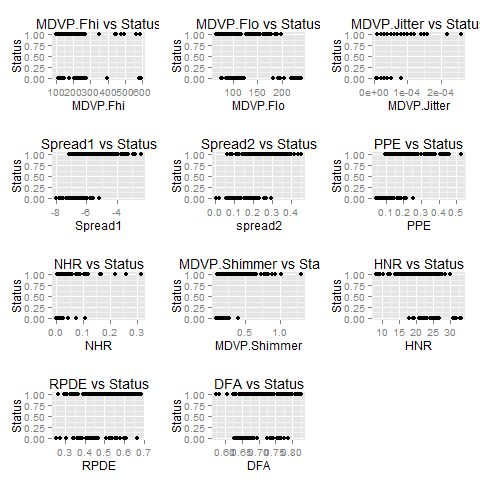
\includegraphics[width=0.6\textwidth]{figures/parkinson.png}
  \caption{Scatter plots for Parkinson data}
  \label{fig:parkinson_scatters}
\end{figure}

\begin{figure}[h]
  \centering
  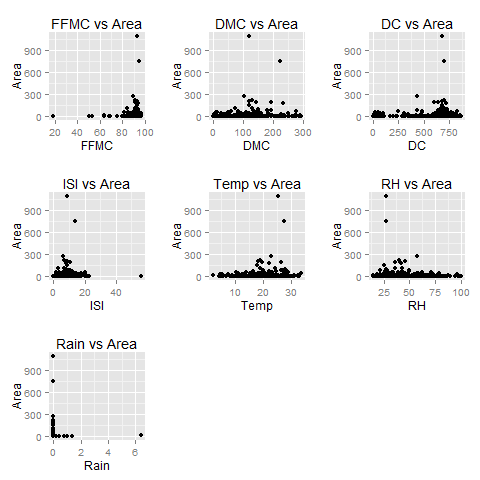
\includegraphics[width=0.6\textwidth]{figures/forestfire.png}
  \caption{Scatter plots for forest fire data}
  \label{fig:fire_scatters}
\end{figure}

\section{Code}
\subsection{Problem 1}
\lstinputlisting[caption=Analysis for Forest Fire Data Set]{p1.R}
\subsection{Problem 2}
\lstinputlisting[caption=Analysis for Parkinson's Data Set]{p2.R}

\section{Who did what}
\begin{itemize}
	\item Aaron - implemented R functions for Problem 1 and 2 and did initial analysis; generated plots
	\item Anatoly - assisted Aaron in development of Problem 1 and 2 code
	\item Justin - used Devanbu's article to finish Problem 3; generated plots
	\item Samuel - wrote R to do analysis/plots, copy-edited Problem 3 and did write-up for Problem 1 and 2
\end{itemize}

\end{document}             % End of document.
